\documentclass{article}\usepackage{amsmath,amsfonts,amssymb}
\usepackage[utf8]{inputenc}
\usepackage{polski}
\usepackage[polish]{babel}
\usepackage[T1]{fontenc}
\usepackage[dvips]{graphicx}
\usepackage{natbib}
\usepackage{setspace}
\usepackage{graphicx}
\usepackage{xcolor}
\usepackage{enumerate}
\usepackage{fancyhdr}
\usepackage{mathtools}
\usepackage{extarrows}
\usepackage{relsize}
\usepackage[hmargin=2cm, vmargin=2cm, hcentering]{geometry}
\usepackage{subfig}
\usepackage{tocloft}
\usepackage{arydshln} % \hdashline
\usepackage[table]{xcolor}
\usepackage[table, dvipsnames]{xcolor}
\usepackage{booktabs}% http://ctan.org/pkg/booktabs
\newcommand{\tabitem}{~~\llap{\textbullet}~~}
\usepackage{enumitem}
\usepackage{caption}
\usepackage{listings}

% \usepackage{tocstyle}
% \usetocstyle{standard}
% \settocfeature{raggedhook}{\raggedright}

\newlist{todolist}{itemize}{2}
\setlist[todolist]{label=}
% \renewcommand\labelitemi{$\square$}

\usepackage{hyperref}
% \hypersetup{
%     colorlinks,
%     citecolor=black,
%     filecolor=black,
%     linkcolor=black,
%     urlcolor=black
% }
% \pagestyle{fancy}
% \fancyhf{}
\doublespacing

\title{Projekt nr 1 \\}
\author{Michał Piasecki gr 1. }


\begin{document}

\maketitle

\section{Temat i treść zadania}
W poniższej pracy zajmiemy się problemem badania przybliżonej wartości całki z wielomianów postaci: \[ w_{n}(x) = \sum_{k = 0}^{n} a_{k}  \cdot T_{k}(x)  \cdot U_{k}(x) \] 
\boldmath
$a_{k}$ - ciąg wartości \\
$T_{k}(x)$ - wielomian Czebyszewa pierwszego rzędu \\
$U_{k}(x)$ - wielomian Czebyszewa drugiego rzędu \\
\unboldmath
Wielomiany Czebyszewa definiuje się w następny sposób: \\
\\
Wielomian Czebyszewa pierwszego rodzaju:
\[ T_{0}(x) = 1 \] 
\[ T_{1}(x) = x \] 
\[ T_{n}(x) = 2 \cdot x \cdot T_{n - 1}(x) - T_{n - 2}(x) \quad  \forall  n \geq 2 \] 
Wielomian Czebyszewa drugiego rodzaju:
\[ U_{0}(x) = 1 \] 
\[ U_{1}(x) = 2 \cdot x \] 
\[ U_{n}(x) = 2 \cdot x \cdot U_{n - 1}(x) - U_{n - 2}(x) \quad  \forall  n \geq 2 \] 


\newpage
\section{Metoda trapezów}
Aby policzyć przybliżoną wartość całki z naszych wielomianów posłużymy się złożoną kwadraturą trapezów. \\ 
Wprowadźmy oznaczenia : \\
\boldmath
$f(x)$ - nasza funkcja, z której chcemy policzyć całkę \\ 
$[a, b]$ -  przedział na którym chcemy naszą funkcję scałkować \\
$N$ - parametr mówiący ile węzłów chcemy użyc do policzenia przybliżonej wartości całki \\ 
$E$ - błąd popełniany przy mierzeniu pola metodą trapezów
\unboldmath
Przedział $[a, b]$ dzielimy na podprzedziały $[x_{k−1}, x_{k}] \quad (k = 1, . . . , N)$, o długości $H =(b−a)/N$,
przy czym $xk = a+kH $ dla $k = 0, . . . , N$. Na każdym podprzedziale stosujemy kwadraturę prostą.\\
Otrzymujemy przybliżoną wartość naszej całki:
\[ S(f) = \sum_{k=1}^{N}\frac{(x_{k} - x_{k - 1})}{2}  (f(x_{k} + f(x_{k - 1})) \] 
A po przekształceniu otrzymujemy:
\[ S(f) = \frac{H}{2}(f(a) + f(b) +  2\cdot\sum_{k=1}^{N-1}f(a + kH)\] 
Oczywiście pojawia się pytanie jaki błąd popełniamy przy mierzeniu całki taką metodą. Okazuje się, że
\[ E(f) = -\frac{1}{12}H^2(b-a)f''(\alpha) \quad \alpha \in [a,b]\] 
więc oczywiście zachodzi:
\[ \lvert E(f) \rvert \leq \lvert\frac{1}{12}H^2(b-a)max_{[a,b]}(f''(x) \rvert \] 
\begin{center}
   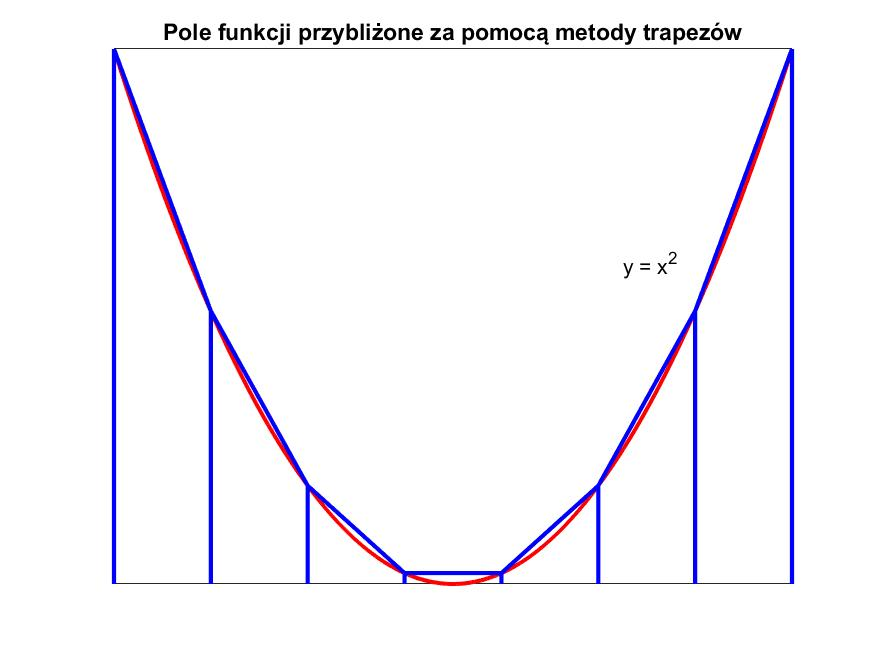
\includegraphics[scale=0.3]{kwadratowa_1.jpg}
\end{center}

\newpage
\section{Opis programu obliczeniowego}
Funkcja, która realizuje obliczanie całki z funkcji nazywa sie $calkaTrapezowa(f,a,b,n)$ \\
\textbf{Argumenty}: \\
$f$ - funkcja, którą całkujemy \\
$a$ - początek przedziału całkowania \\
$b$ - koniec przedziału całkowania  \\
$n$ - ilość węzłów \\
\textbf{Działanie funkcji}: \\
Funkcja wyznacza zmienną pomocniczą $h = \frac{b - a}{n}$. Następnie dzieli przedział $[a,b]$ na n-równych podprzedziałów  o dlugości $h$. Następnie sumuje $n - 1$ trapezów utworzonych z wartości funkcji na poszczególnych podprzedziałach oraz zwraca maksymalną wartość błędu.

\lstset{language=Matlab,%
    %basicstyle=\color{red},
    breaklines=true,%
    morekeywords={matlab2tikz},
    keywordstyle=\color{blue},%
    morekeywords=[2]{1}, keywordstyle=[2]{\color{black}},
    identifierstyle=\color{black},%
    stringstyle=\color{mylilas},
    commentstyle=\color{mygreen},%
    showstringspaces=false,%without this there will be a symbol in the places where there is a space
    numbers=left,%
    numberstyle={\tiny \color{black}},% size of the numbers
    numbersep=9pt, % this defines how far the numbers are from the text
    emph=[1]{for,end,break},emphstyle=[1]\color{red}, %some words to emphasise
    %emph=[2]{word1,word2}, emphstyle=[2]{style},    
}
\lstinputlisting{CroutLU.m}


\section{Ciekawe przykłady obliczeniowe}
Wygenerujmy różne wielomiany $w_{n}(x)$ i zobaczmy jak sprawdza się nasza metoda w porównaniu z liczeniem całki symbolicznie. \\
Niech:
\[ w_{n}(x) = \sum_{k = 0}^{2} a_{k}  \cdot T_{k}(x)  \cdot U_{k}(x) \quad \quad a_{k} = k +1 \] 
\newpage
Nasza funkcja wygląda tak:
\begin{center}
   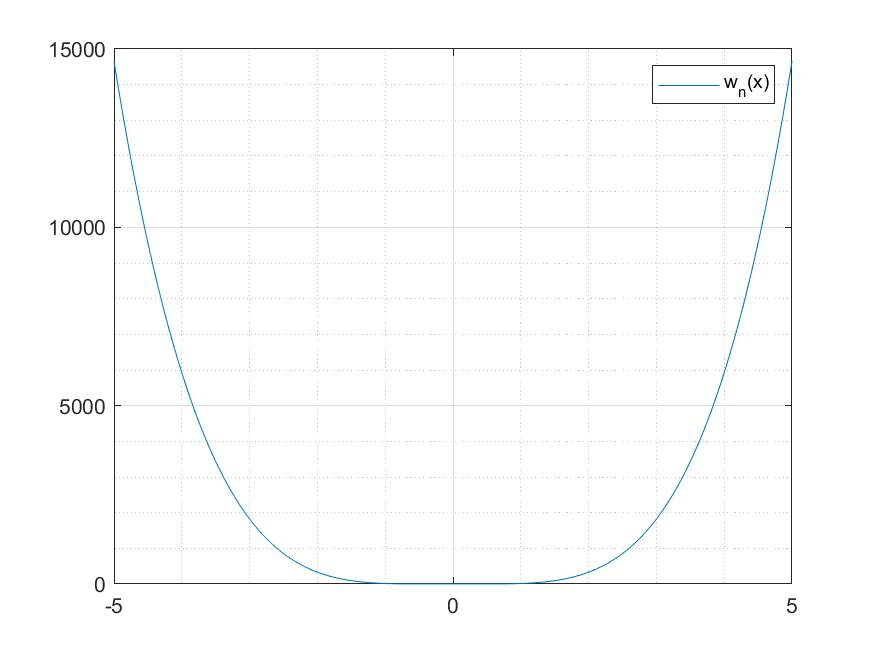
\includegraphics[scale=0.3]{drugi_rysunek.jpg}
\end{center}
Policzmy całkę na przedziale $[0, 5]$. Weźmy kolejno 2, 7 oraz 100 węzłów.
otrzymujemy kolejno: \\
\[ S(w_{n}, 0, 5, 3) = 1072.5 \] 
\[ S(w_{n}, 0, 5, 7) = 6905.1 \] 
\[ S(w_{n}, 0, 5, 1000) = 14364 \] 
\[ \int_0^5w_n(x)dx \approx 14436 \] 
Widzimy więc, że dopiero przy wzięciu sporej ilości węzłów nasza metoda w jakikolwiek sensowny sposób przybliża nam wartość całki.\\
Zobaczmy czy jeśli zmniejszymy przedział $[a,b]$ to pozwoli nam to wziąć dużo mniej węzłów aby uzyskać sensowny wynik. 
Zobaczmy:
\[ S(w_{n}, 0, 1, 15) = 7.51 \] 
\[ \int_0^1w_n(x)dx = 8.26 \] 
Już przy 15 węzłach osiągneliśmy całkiem zbliżony wynik.
Możemy domyślać się, że wynika to z tego, że funkcja $w_n(x)$ rośnie bardzo szybko przez co im dalszy zakres od zera weźmiemy tym więcej potrzebujemy węzłów, żeby w przybliżony sposób osiągnąć pole. Ponadto przy mniejszych wartościach funkcji błędy, które popełniamy są bezwględnie mniejsze. \\
Weźmy teraz wielomian który będzie tylko iloczynem wielomianów Czeryszewa 4 stopnia tzn.
\[ w_{n}(x) = \sum_{k = 0}^{4} a_{k}  \cdot T_{k}(x)  \cdot U_{k}(x) \quad \quad a_{i} = \left \lfloor{\frac{i}{4}}\right \rfloor  \] 
\[ w_{n}(x) =  T_{4}(x)  \cdot U_{4}(x)   \] 
\begin{center}
   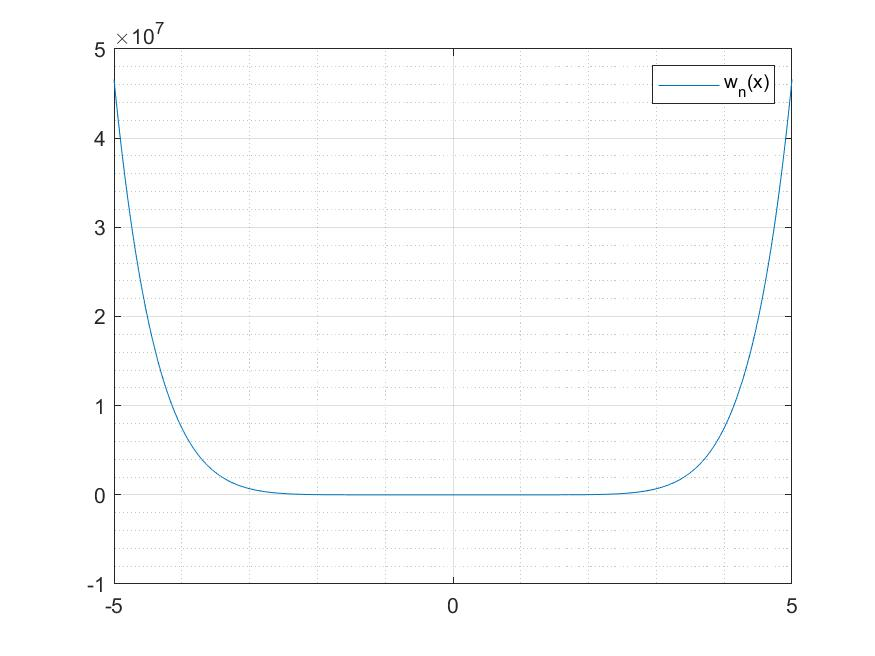
\includegraphics[scale=0.3]{trzeci_rysunek.jpg}
\end{center}
Ta funkcja to nam już totalnie eksploduje. Zobaczmy czy przybliżenie na 1000 węzłów będzie blisko poprawnego wyniku:
Mamy:
\[ S(w_{n}, 0, 5, 1000) = 2.512 \cdot10^7 \] 
\[ \int_0^5w_n(x)dx = 2.53\cdot10^7\] 


Zmniejszymy teraz współczynniki przy naszym wielomianie. Policzmy $w_{n}(x)$ na przedziale $[-3,3]$
\[ w_{n}(x) = \sum_{k = 0}^{4} a_{k}  \cdot T_{k}(x)  \cdot U_{k}(x) \quad \quad a_{k} = \frac{1}{10^{k+1}}\] 
\begin{center}
   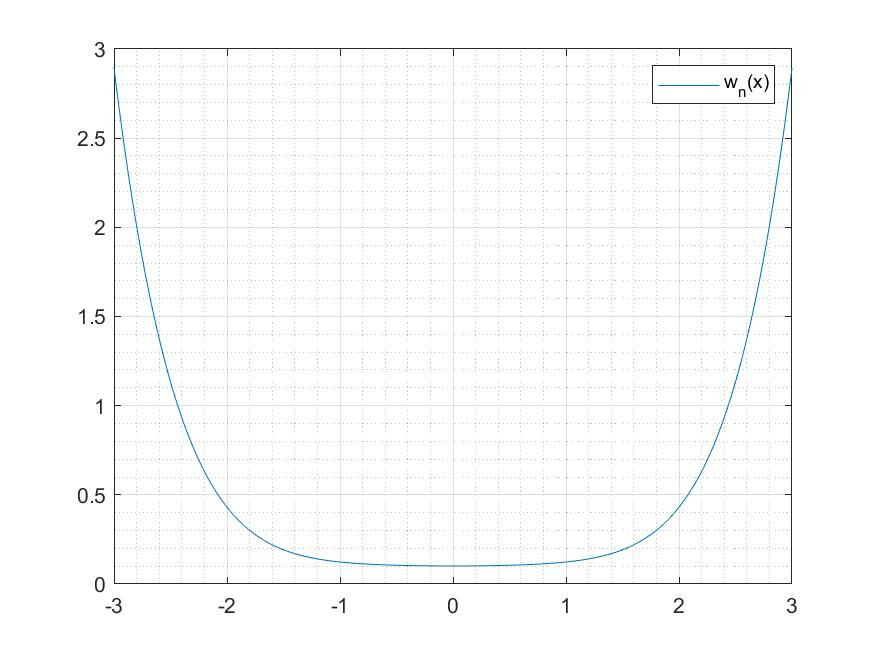
\includegraphics[scale=0.3]{obrazek_4.jpg}
\end{center}
Mamy:
\[ S(w_{n}, -3, 3, 5) = 2.5358  \] 
\[ S(w_{n}, -3, 3, 20) =  2.6617  \] 
\[ S(w_{n}, -3, 3, 100) =  3.1063  \] 
\[ \int_-3^3w_n(x)dx = 3.26\] 

Zastanówmy sie jeszcze nad tym jak szybko wykonuje sie obliczenie metodą trapezów . Niech:
\[ w_{n}(x) = \sum_{k = 0}^{6} a_{k}  \cdot T_{k}(x)  \cdot U_{k}(x) \quad \quad a_{k} = \frac{1}{10^{k+1}}\] 
Mamy:\\
\boldmath
$S(w_{n}, -5, 5, 10) $  -   Elapsed time is 0.001467 seconds.\\
$ S(w_{n}, -5, 5, 100) $  - Elapsed time is 0.010243 seconds.\\
\unbold math
Wróćmy do naszego przykładu pierwszego:
\[ w_{n}(x) = \sum_{k = 0}^{2} a_{k}  \cdot T_{k}(x)  \cdot U_{k}(x) \quad \quad a_{k} = k +1 \] 
i zobaczmy jakie jest oszacowanie błędu:
\[ \lvert E(f,0,5,7) \rvert \leq 1034.5 \]
\[ \lvert E(f,0,5,100) \rvert \leq 0.374   \] 
\[ \lvert E(f,0,5,1000) \rvert \leq  0.0004\] 
Wygenerujmy więc może funkcję która w zależności od ilości węzłow pokazuje nam wartość błędu: (Oś y jest podana w skali logarytmicznej)
\begin{center}
   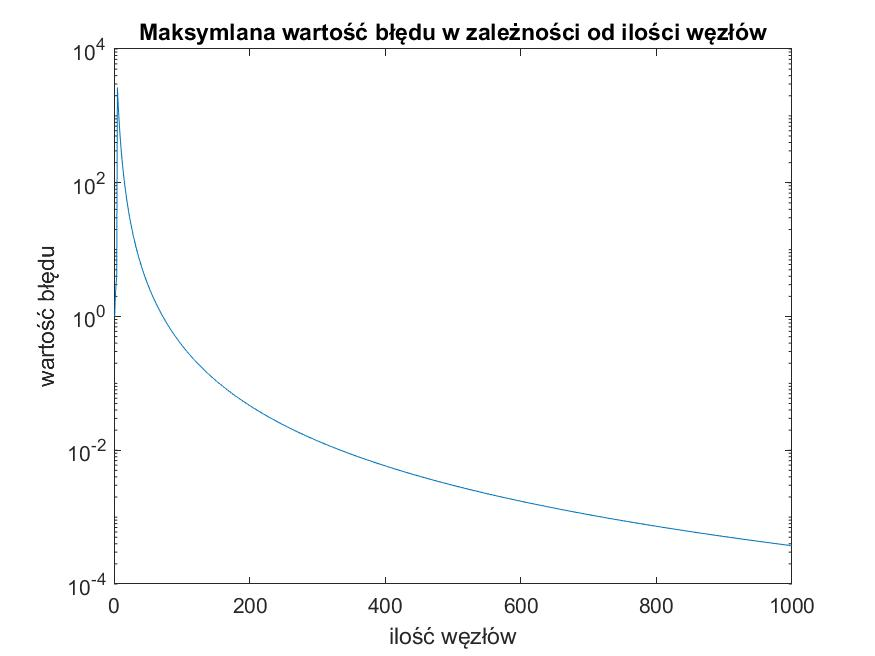
\includegraphics[scale=0.3]{maksymalnebledy.jpg}
\end{center}



\section{Analiza wyników obliczeniowych}
Na podstawie powyższych przykładów widzimy, że aby przybliżyć pole figury metodą trapezów musimy wziąć odpowiednią ilość węzłów.
Wiadome jest, że im więcej węzłów ustalimy tym przybliżona wartość będzie bliższa polu figury.
Oczywiście skoro, wiemy, że \[ \lvert E(f) \rvert \leq \lvert\frac{1}{12}H^2(b-a)max_{[a,b]}(f''(x) \rvert \] możemy  zastanowić się nad przybliżoną maksymalną wartością drugiej pochodnej na naszym przedziale i w zależności od tego dobierać ilość węzłów. W naszych przypadkach mieliśmy do czynienia z funkcjami, które przyrastały bardzo szybko, przez co nieznaczne zwiększanie przedziału całkowania powodowało, że musieliśmy dobierać dużo większą ilość węzłów, aby osiągnąć w miarę zbliżony wynik. Wraz ze zwiększaniem ilości węzłów na danym przedziale, czas wykonywania naszej funkji będzie rósł w czasie liniowym.]






















\end{document}
